\documentclass[letterpaper,final,12pt,reqno]{amsart}

\usepackage[total={6.3in,9.2in},top=1.1in,left=1.1in]{geometry}

\usepackage{verbatim}
\usepackage{empheq}
\usepackage[dvipsnames]{xcolor}
\usepackage{animate}
\usepackage{graphicx}
\usepackage{fancyvrb}

%\usepackage{palatino}

% hyperref should be the last package we load
\usepackage[pdftex,
colorlinks=true,
plainpages=false, % only if colorlinks=true
linkcolor=blue,   % only if colorlinks=true
citecolor=Red,   % only if colorlinks=true
urlcolor=black     % only if colorlinks=true
]{hyperref}

\renewcommand{\baselinestretch}{1.05}

\newcommand{\ddt}[1]{\ensuremath{\frac{\partial #1}{\partial t}}}
\newcommand{\ddx}[1]{\ensuremath{\frac{\partial #1}{\partial x}}}
\newcommand{\ddy}[1]{\ensuremath{\frac{\partial #1}{\partial y}}}
\newcommand{\pp}[2]{\ensuremath{\frac{\partial #1}{\partial #2}}}
\renewcommand{\t}[1]{\texttt{#1}}
\newcommand{\Matlab}{\textsc{Matlab}\xspace}
\newcommand{\eps}{\epsilon}
\newcommand{\RR}{\mathbb{R}}

\newcommand{\grad}{\nabla}
\newcommand{\Div}{\nabla\cdot}
\newcommand{\trace}{\operatorname{tr}}


\newcommand{\hbn}{\hat{\mathbf{n}}}

\newcommand{\bg}{\mathbf{g}}
\newcommand{\bu}{\mathbf{u}}
\newcommand{\bv}{\mathbf{v}}

\newcommand{\bX}{\mathbf{X}}



\begin{document}
\graphicspath{{../figures/}}

\title[Appendix A: A finite element Stokes solver for glacier flow]{Appendix A: A finite element Stokes solver \\ for glacier flow}

\author{Ed Bueler}

\date{\today}

\maketitle

\renewcommand{\theequation}{A\arabic{equation}}


This document is an appendix to my notes \emph{Numerical modelling of glaciers, ice sheets, and ice shelves}---here called ``the notes''---which are used for the International Summer School in Glaciology in McCarthy, Alaska.

We start by stating the Stokes model with glacier-suitable boundary conditions.  Then we derive the ``weak form,'' as explained below.  A finite element (FE) method \cite{Elmanetal2014} is based on this weak form.  An overview of our FE method follows; it uses triangular elements for an arbitrary planar region.  We briefly discuss choosing stable mixed elements for the Stokes problem.  We construct slab-on-a-slope solutions both for verification and to clarify the boundary conditions.  Then we describe how four open-source tools/libraries are using to generate a numerical solution:
\begin{itemize}
\item Gmsh, a mesh generator \hfill \url{http://gmsh.info/}
\item Firedrake, an FE library \hfill \url{https://www.firedrakeproject.org/}
\item PETSc, a solver library \hfill \url{http://www.mcs.anl.gov/petsc/}
\item Paraview, visualization tool \hfill \url{https://www.paraview.org/}
\end{itemize}
These notes end by demonstrating a relatively-short Python code.

\section{Stokes equations and their weak form}

Recall the Glen-Stokes model in equations (3), (4), (5) from the notes---it is also stated in \cite{GreveBlatter2009,JouvetRappaz2011}.  Allowing any Glen exponent $n\ge 1$, the equations are:
\begin{align}
\nabla \cdot \bu &= 0 &&\text{\emph{incompressibility}} \label{incompressible} \\
- \nabla \cdot \tau + \nabla p &= \rho \bg &&\text{\emph{stress balance}} \label{forcebalance} \\
D\bu &= A_n |\tau|^{n-1} \tau &&\text{\emph{Glen flow law}} \label{flowlaw}
\end{align}
The velocity $\bu$, pressure $p$, ice density $\rho$, acceleration of gravity $\bg$, deviatoric stress tensor $\tau$ and strain rate tensor $D\bu$ all appear.  Note that $A_n$ in \eqref{flowlaw} is the $n$-dependent ice softness.  The model applies on a 3D domain $\Omega\subset \RR^3$ or 2D domain $\Omega \subset \RR^2$ according to the context.

Though the notation here generally follows Table 1 in the notes, some of usage is more general or flexible.  For example, Table 1 shows $A = A_3 = 10^{-16} \,\text{Pa}^{-3}\,\text{a}^{-1} = 3.1689 \times 10^{-24} \,\text{Pa}^{-3}\,\text{s}^{-1}$, but generally the units of $A_n$ are $\text{Pa}^{-n}\,\text{s}^{-1}$.

Regarding tensors and their norms we have:
\begin{align*}
(D\bu)_{ij} &= \frac{1}{2} \left((u_i)_{x_j} + (u_j)_{x_i}\right) \\
|\tau|^2 &= \frac{1}{2} \trace\left(\tau^\top \tau\right) = \frac{1}{2} \tau_{ij} \tau_{ij} \\
|D\bu|^2 &= \frac{1}{2} \trace\left((D\bu)^\top D\bu\right) = \frac{1}{2} (D\bu)_{ij} (D\bu)_{ij}
\end{align*}
In the last two expressions the Einstein summation is used, either over indices $i,j=1,2,3$ or $i,j=1,2$ according to dimension.  Note that the tensors $D\bu$ and $\tau$ are symmetric and have trace zero.  Also, the full (Cauchy) stress tensor $\sigma$ is the deviatoric stress tensor $\tau$ minus the pressure,
\begin{equation}
    \sigma = \tau - p\,I,  \label{cauchystress}
\end{equation}
so equation \eqref{forcebalance} may be written as $-\Div \sigma = \rho \bg$.  One may derive from \eqref{cauchystress} that $p = -\frac{1}{3} \trace(\sigma)$, because $\tau$ has trace zero, thus that the pressure is the negative of the average normal stress.  Finally, by definition the divergence of the tensor $\tau$ has components which we regard as the divergences of the rows:
    $$\left(\nabla \cdot \tau\right)_i = \left(\tau_{i1}\right)_{x_1} + \left(\tau_{i2}\right)_{x_2} + \left(\tau_{i3}\right)_{x_3},$$
Then $\nabla\cdot \tau$ would be a column vector, necessarily like $\nabla p$ and $\bg$ in \eqref{forcebalance}.

Recall the viscosity form of flow law \eqref{flowlaw}, namely equation (15) in the notes:
\begin{equation}
\tau = 2\nu D\bu = B_n |D\bu|^{\frac{1}{n} - 1} D\bu  \label{viscflowlaw}
\end{equation}
Here $B_n = A_n^{-1/n}$ is the $n$-dependent ice hardness.  With this expression we can eliminate $\tau$ and rewrite equations \eqref{incompressible}, \eqref{forcebalance} as
\begin{align}
\Div \bu &= 0 \label{incompagain} \\
- \nabla \cdot \left(B_n |D\bu|^{\frac{1}{n} - 1} D\bu\right) + \nabla p &= \rho \mathbf{g} \label{stokes}
\end{align}
The Stokes model in strong form is, from now on, equations \eqref{incompagain}, \eqref{stokes} with certain boundary conditions, and the solution is the velocity-pressure pair $(\bu,p)$.

The domain $\Omega$ must have a smooth-enough boundary to apply the boundary conditions but it is otherwise general.  To explain the boundary conditions consider the numerical solution shown in Figure \ref{fig:stepflowlin}.  The particular problems solved here will have well-defined base, top, inflow, and outflow boundary surfaces.  On the base we set a Dirichlet condition of no slip:
\begin{align*}
\bu &= 0  &&\text{(\emph{base})} \\
\intertext{On the top we set a condition of zero normal stress, $\sigma\hbn=0$ or equivalently:}
\left(B_n |D\bu|^{\frac{1}{n} - 1} D\bu - pI\right) \hbn &= 0  &&\text{(\emph{top})} \\
\intertext{On the inflow boundary, the left side in Figure \ref{fig:stepflowlin}, a surface with outward normal $\hbn=\left<-1,0,0\right>^\top$ in the cases we solve, we set a nonzero inflow (normal) Dirichlet condition:}
\bu &= \left<f(z),0,0\right>^\top  &&\text{(\emph{inflow})}
\intertext{The inflow function $f(z)$ will be defined later as satisfying the slab-on-slope equations.  Finally for the outflow boundary we se a nonzero normal stress condition bases on assuming hydrostatic normal stress:}
\left(B_n |D\bu|^{\frac{1}{n} - 1} D\bu - pI\right) \hbn &= \left<-\rho g (h-z),0,0\right>^\top  &&\text{(\emph{outflow})}
\end{align*}
where the outward normal is $\hbn=\left<1,0,0\right>^\top$, $h$ is the surface elevation, and $g=|\bg|$.

\begin{figure}
\label{fig:stepflowlin}
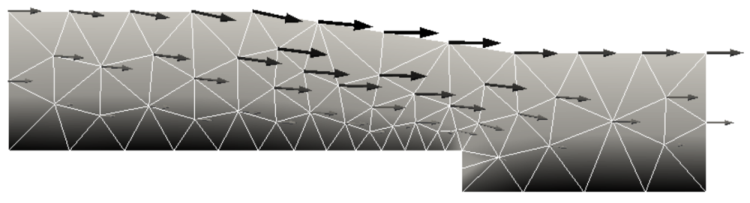
\includegraphics[width=0.95\textwidth]{stepflowlin}
\caption{A 2D Stokes problem for a glacier flowing over a bedrock step.  Arrows show velocity $\bu$ and shading is by pressure $p$.  Note the (coarse) mesh of triangular finite elements.}
\end{figure}

The solution is the pair $(\bu,p)$ where $\bu\in V_D$ and $p \in Q$ for function spaces $V_D,Q$ precisely identified in \cite{JouvetRappaz2011}.  The weak formulation is derived by multiplying the equations by arbitrary test functions, from nearly the same spaces as the solution, to define a nonlinear functional $F$.  Specifically we multiply \eqref{incompressible} by test function $q\in Q$ and \eqref{stokes} by test function $\bv\in V_0$, and we combine:
\begin{equation}
F(\bu,p;\bv,q) = \int_\Omega - \left(\nabla \cdot \left(B_n |D\bu|^{\frac{1}{n} - 1} D\bu\right)\right)\cdot \bv + \nabla p \cdot \bv - \rho \mathbf{g} \cdot \bv - \left(\nabla \cdot \bu\right) q \label{nonfuncone}
\end{equation}
The difference between spaces $V_D$ and $V_0$ only relates to the value of Dirichlet boundary conditions \cite{JouvetRappaz2011}.  The nonlinear functional must be zero at the solution $(\bu,p)$:
\begin{equation}
F(\bu,p;\bv,q) = 0 \qquad \text{ for all } \bv\in V_0 \text{ and } q\in Q
\end{equation}

Integration-by-parts allows the solution (trial) and test functions to actually live in spaces of functions with comparable smoothness, as already claimed.  That is, the nonlinear functional $F$ can be rewritten to use the same number of derivatives on $(\bv,q)$ as appear on $(\bu,p)$.  Recall integration-by-parts combines the product rule $\nabla \cdot(f\bX) = \grad f\cdot \bX + f \nabla \cdot \bX$ and the divergence theorem $\int_\Omega \nabla \cdot \bX = \int_{\partial \Omega} \bX \cdot \hbn$.  Denoting $\tau = B_n |D\bu|^{\frac{1}{n} - 1} D\bu$ for simplicity,
\begin{align*}
\int_\Omega \left(\nabla \cdot \tau\right)\cdot \bv &= \sum_{j=1}^3 \int_\Omega \nabla \cdot (\tau_{j\circ})\, v_j = \sum_{j=1}^3 \int_\Omega \nabla \cdot (\tau_{j\circ} v_j) - \tau_{j\circ} \nabla v_j \\
  &= \sum_{j=1}^3 \int_{\partial \Omega} (\tau_{j\circ} v_j) \cdot \hbn - \int_\Omega \tau_{j\circ} \nabla v_j = \int_{\partial \Omega} (\tau \hbn)\cdot \bv - \int_\Omega \tau \cdot \nabla \bv
\end{align*}
where $\circ$ denotes an index iterated-over, and similarly
    $$\int_\Omega \nabla p \cdot \bv = \int_\Omega \nabla\cdot (p\,\bv) - p (\nabla \cdot \bv) = \int_{\partial \Omega} (p I\hbn)\cdot \bv - \int_\Omega p (\nabla \cdot \bv)$$
These expressions allow us to rewrite \eqref{nonfuncone} with an integral of the normal stress over the boundary:
\begin{align}
F(\bu,p;\bv,q) &= -\int_{\partial\Omega} ((\tau-pI) \hbn)\cdot \bv + \int_\Omega \tau \cdot \nabla \bv - p (\nabla \cdot \bv) - \rho \mathbf{g} \cdot \bv - \left(\nabla \cdot \bu\right) q \label{nonfunctwo}
\end{align}

The weak formulation of the model, as follows, is proven in \cite{JouvetRappaz2011} to be well-posed under reasonable assumptions which will be satisfied in the cases we consider.




\footnotesize

\bigskip
%from: \bibliographystyle{siam}

\begin{thebibliography}{6}

\bibitem{BaliseRaymond1985}
{\sc M.~Balise and C.~Raymond}, {\em Transfer of basal sliding variations to
  the surface of a linearly-viscous glacier}, J. Glaciol., 31 (1985),
  pp.~308--318.

\bibitem{Brownetal2013}
{\sc J.~Brown, B.~Smith, and A.~Ahmadia}, {\em Achieving textbook multigrid
  efficiency for hydrostatic ice sheet flow}, SIAM J. Sci. Computing,
  35 (2013), pp.~B359--B375.

\bibitem{Elmanetal2014}
{\sc H.~C. Elman and D.~J. Silvester and A.~J. Wathen}, {\em Finite Elements
  and Fast Iterative Solvers: with Applications in Incompressible Fluid Dynamics},
  Oxford University Press, 2nd~ed., 2014.

\bibitem{GreveBlatter2009}
{\sc R.~Greve and H.~Blatter}, {\em Dynamics of {I}ce {S}heets and {G}laciers},
  Advances in Geophysical and Environmental Mechanics and Mathematics,
  Springer, 2009.

\bibitem{JouvetRappaz2011}
{\sc G.~Jouvet and J.~Rappaz}, {\em Analysis and finite element approximation
  of a nonlinear stationary {S}tokes problem arising in glaciology}, Advances
  in Numerical Analysis, (2011).

\bibitem{Lengetal2012}
{\sc W.~Leng, L.~Ju, M.~Gunzburger, S.~Price, and T.~Ringler}, {\em A parallel
  high-order accurate finite element nonlinear {S}tokes ice sheet model and
  benchmark experiments}, J. Geophys. Res., 117 (2012).

\end{thebibliography}


\end{document}
